\chapter{Исследовательская часть}

Для тестирования разработанного алгоритма применялась облачная платформа Google Colab, не требующая установки ПО на локальный компьютер.

\begin{figure}
	\begin{center}
		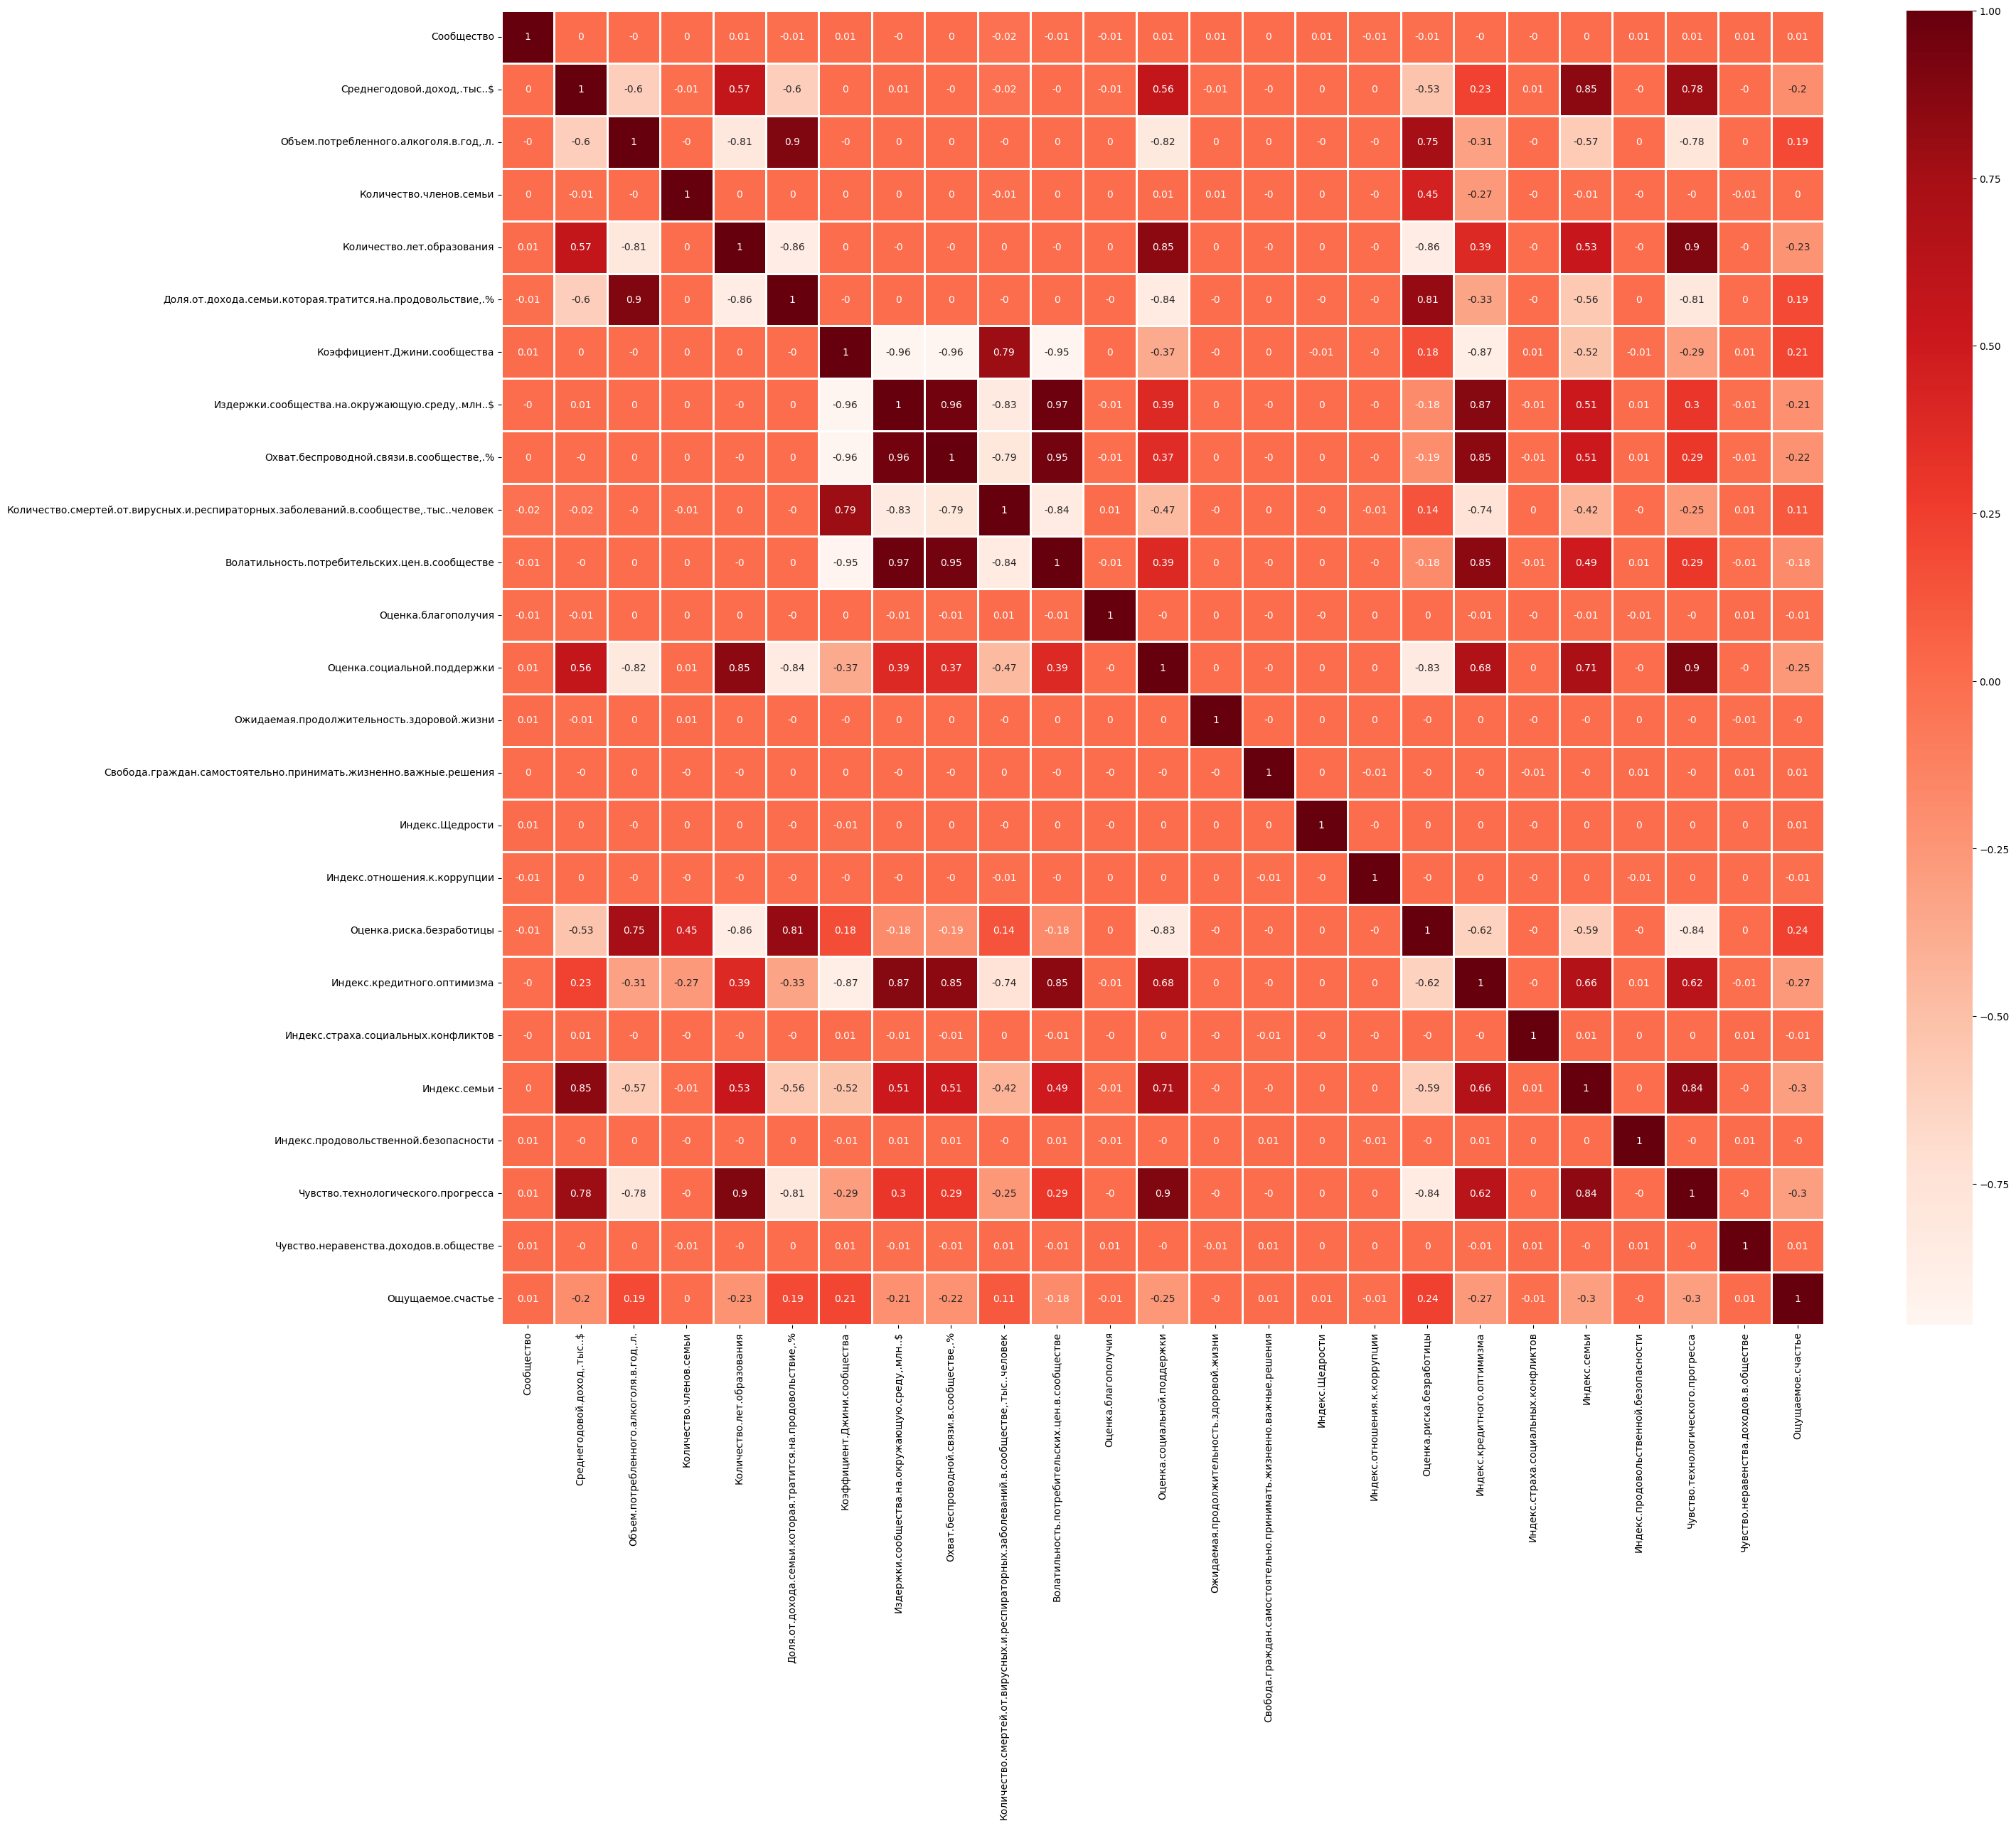
\includegraphics[width=\textwidth]{images/1.png}
	\end{center}
	\caption{Корреляция признаков состояния с интегральной оценкой счастья}
	\label{img:1}
\end{figure}

\begin{figure}
	\begin{center}
		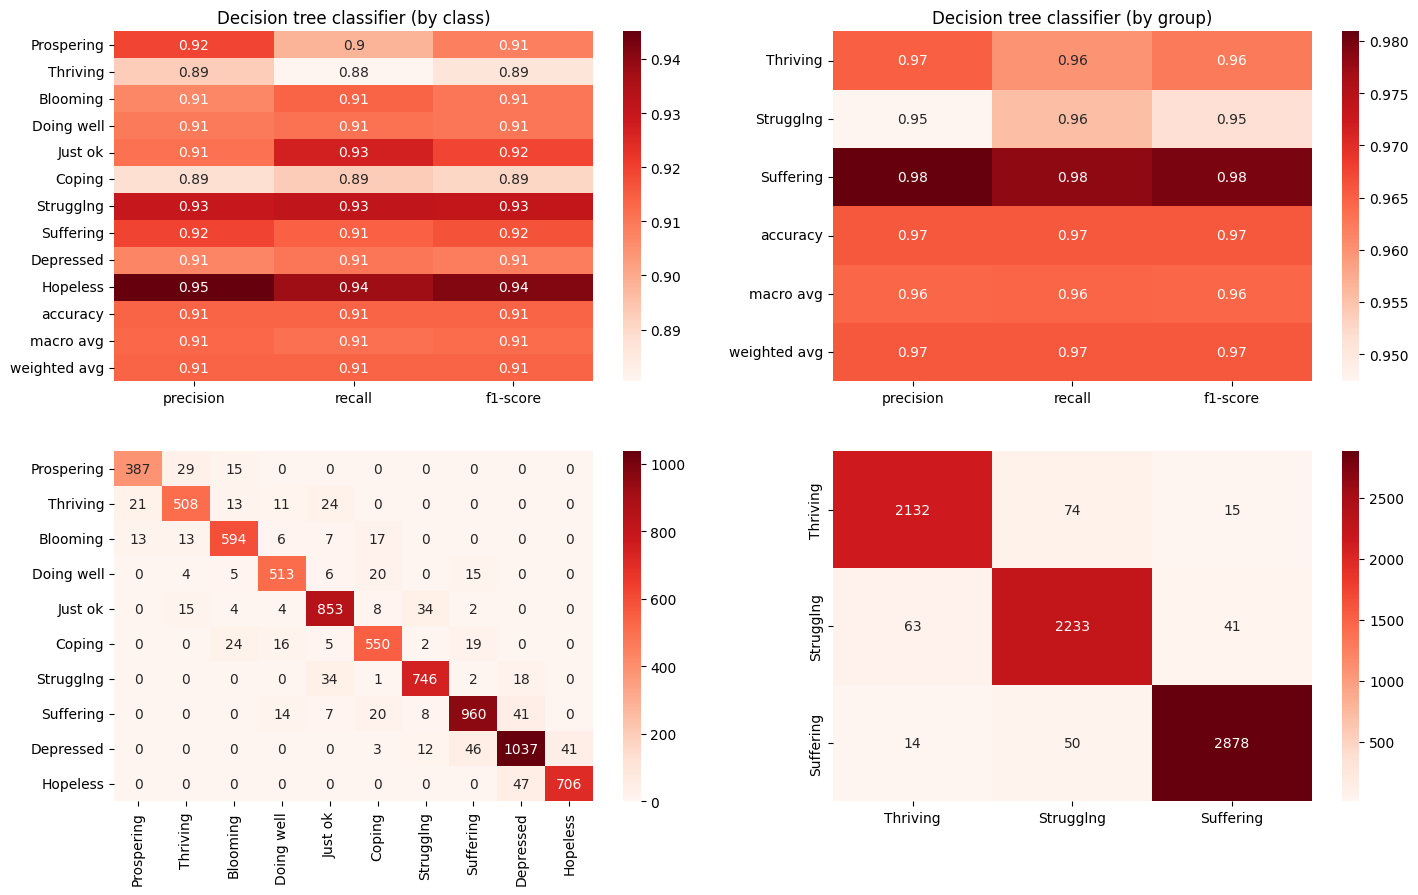
\includegraphics[width=\textwidth]{images/2.png}
	\end{center}
	\caption{Результат классификации с помощью дерева решений (MCC: 0.903)}
	\label{img:2}
\end{figure}

\begin{figure}
	\begin{center}
		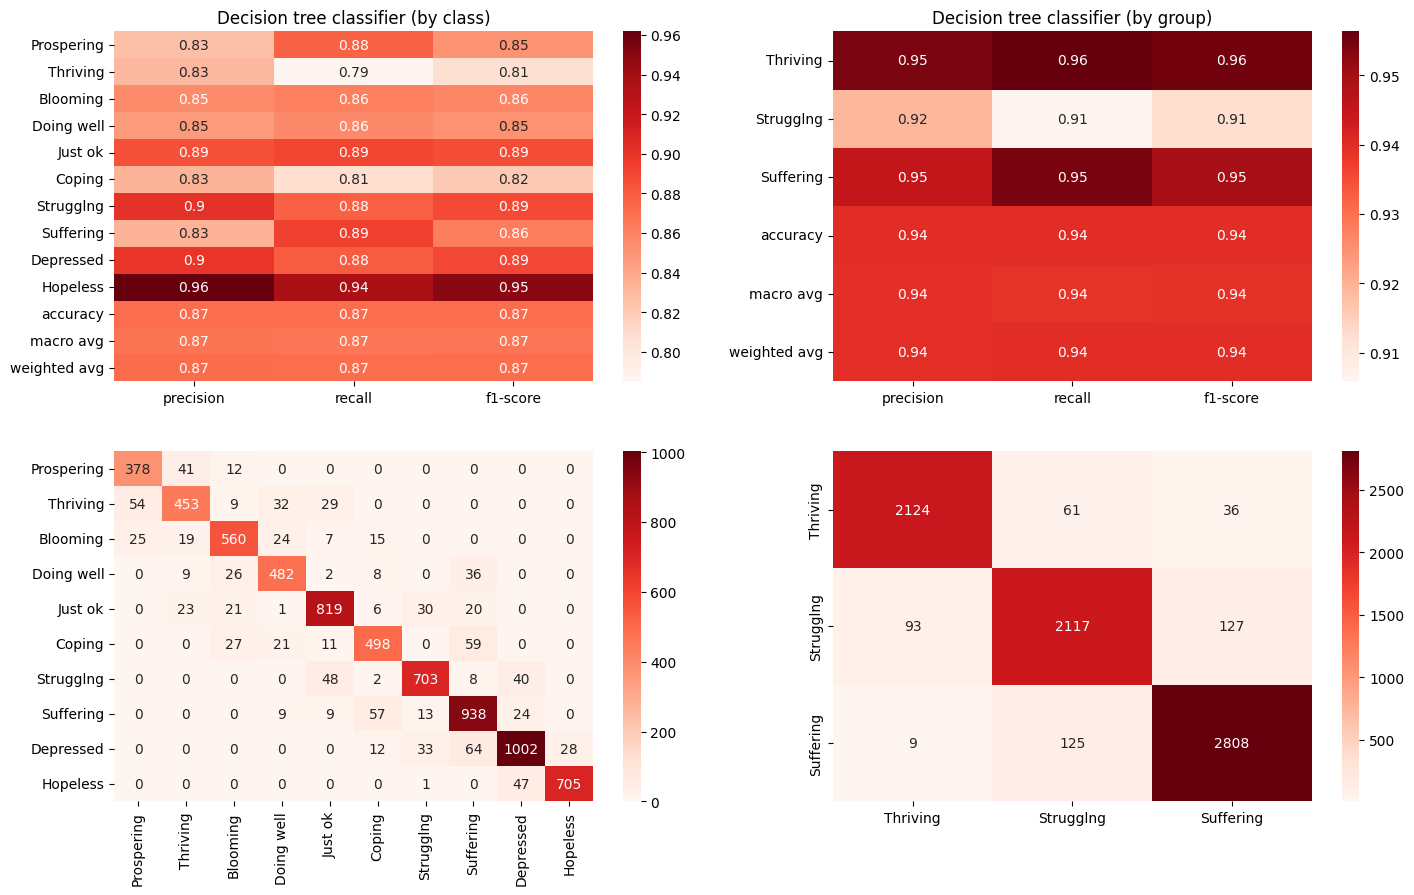
\includegraphics[width=\textwidth]{images/3.png}
	\end{center}
	\caption{Результат классификации с помощью логистической регрессии (MCC: 0.856)}
	\label{img:3}
\end{figure}

\begin{figure}
	\begin{center}
		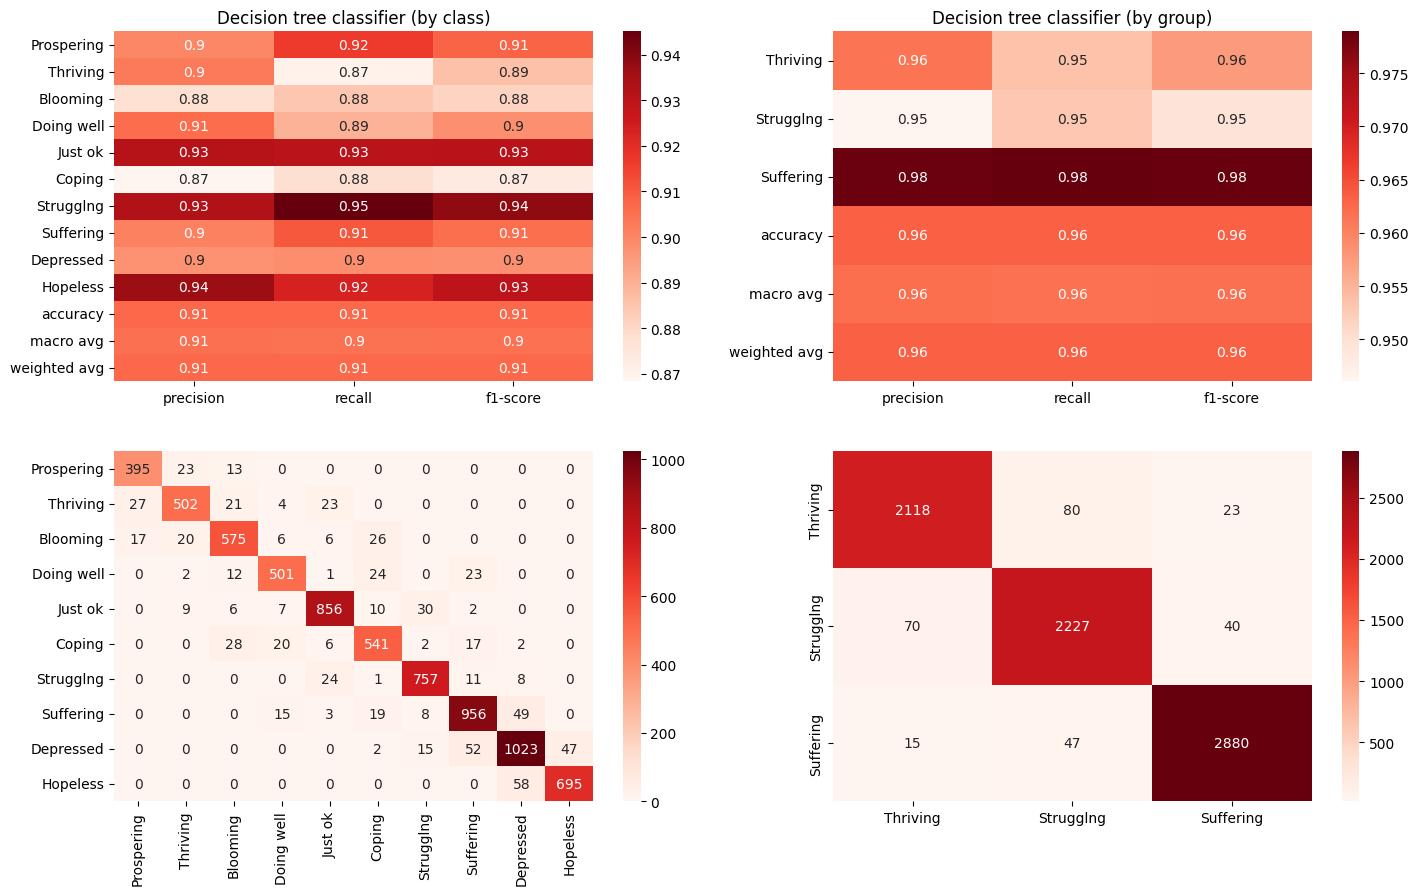
\includegraphics[width=\textwidth]{images/4.png}
	\end{center}
	\caption{Результат классификации с помощью дерева регрессии (MCC: 0.895)}
	\label{img:4}
\end{figure}

\begin{figure}
	\begin{center}
		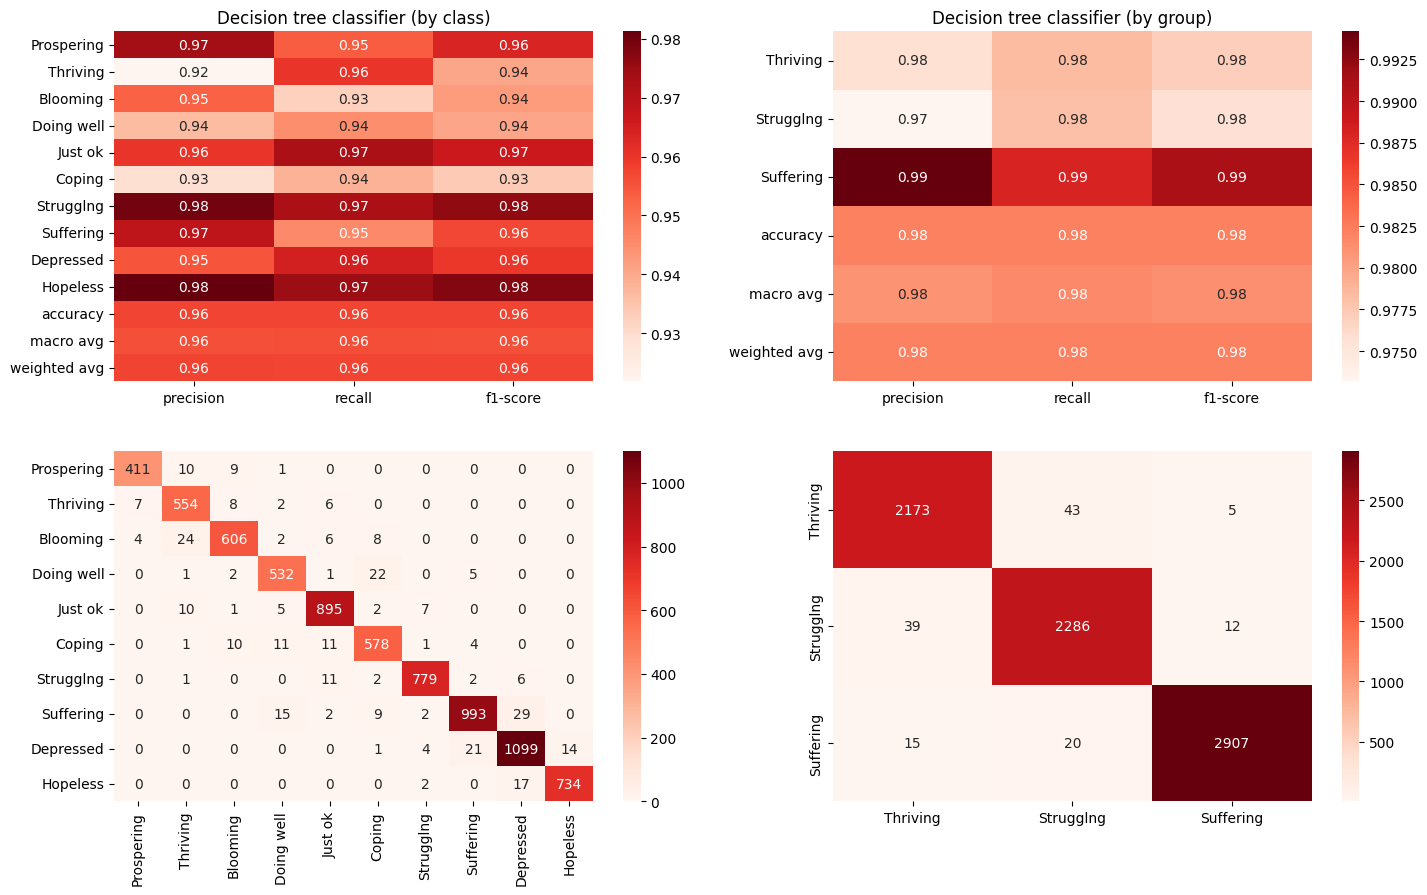
\includegraphics[width=\textwidth]{images/5.png}
	\end{center}
	\caption{Результат классификации с помощью AdaBoost над деревьями регрессии (MCC: 0.952)}
	\label{img:5}
\end{figure}

\clearpage
